\documentclass[letterpaper,11pt]{article}
\usepackage{graphicx}
\usepackage{listings}
\usepackage[super]{nth}
\usepackage[hyphens]{url}
\usepackage{amsmath}
\usepackage[makeroom]{cancel}
\usepackage[table]{xcolor}
\usepackage{comment}
\usepackage[space]{grffile}

\lstset{
	basicstyle=\footnotesize,
	breaklines=true,
}

\begin{document}

\begin{titlepage}

\begin{center}

\Huge{Assignment 6}

\Large{CS 595:  Introduction to Web Science}

\Large{Fall 2013}

\Large{Shawn M. Jones}

\Large Finished on \today

\end{center}

\end{titlepage}

\newpage
\section*{1}

\subsection*{Question}

\begingroup
\fontsize{6pt}{10pt}\selectfont
\begin{verbatim}
1.  We know the result of the Karate Club (Zachary, 1977) split.
Prove or disprove that the result of split could have been predicted
by the weighted graph of social interactions.  How well does the
mathematical model represent reality?

Generously document your answer with all supporting equations, code,
graphs, arguments, etc.

Useful sources include:

* Original paper

http://aris.ss.uci.edu/~lin/76.pdf

* Slides

http://www-personal.umich.edu/~ladamic/courses/networks/si614w06/ppt/lecture18.ppt

http://clair.si.umich.edu/si767/papers/Week03/Community/CommunityDetection.pptx

* Code and data

http://networkx.github.io/documentation/latest/examples/graph/karate_club.html

http://nbviewer.ipython.org/url/courses.cit.cornell.edu/info6010/resources/11notes.ipynb

http://stackoverflow.com/questions/9471906/what-are-the-differences-between-community-detection-algorithms-in-igraph/9478989#9478989

http://stackoverflow.com/questions/5822265/are-there-implementations-of-algorithms-for-community-detection-in-graphs

http://konect.uni-koblenz.de/networks/ucidata-zachary

http://vlado.fmf.uni-lj.si/pub/networks/data/ucinet/ucidata.htm#zachary
\end{verbatim}
\endgroup

\newpage
\subsection*{Answer}

\begin{figure}[h]
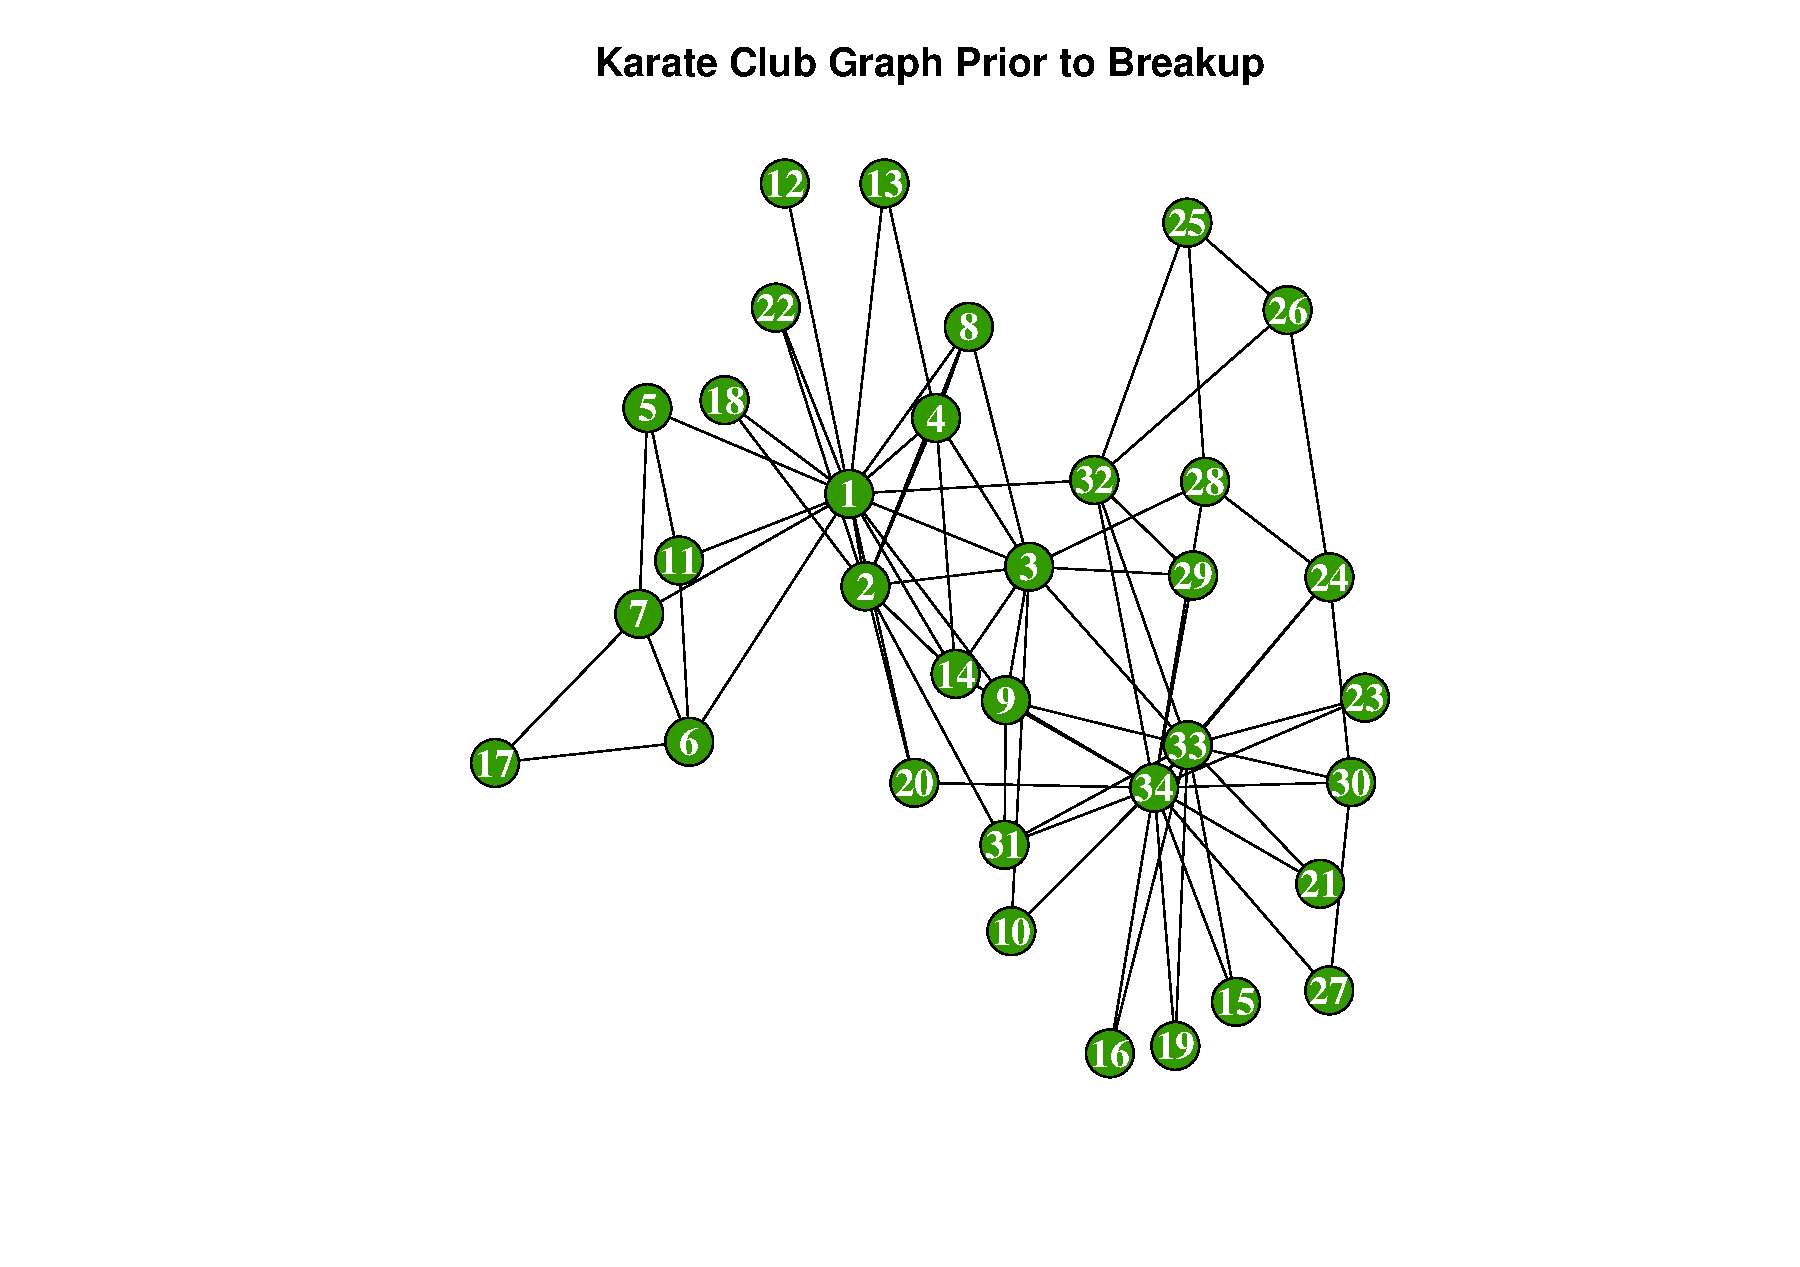
\includegraphics[scale=0.5]{club-before.pdf}
\caption{Karate Club Graph Before Split}
\label{fig:club-before}
\end{figure}

\begin{figure}[h]
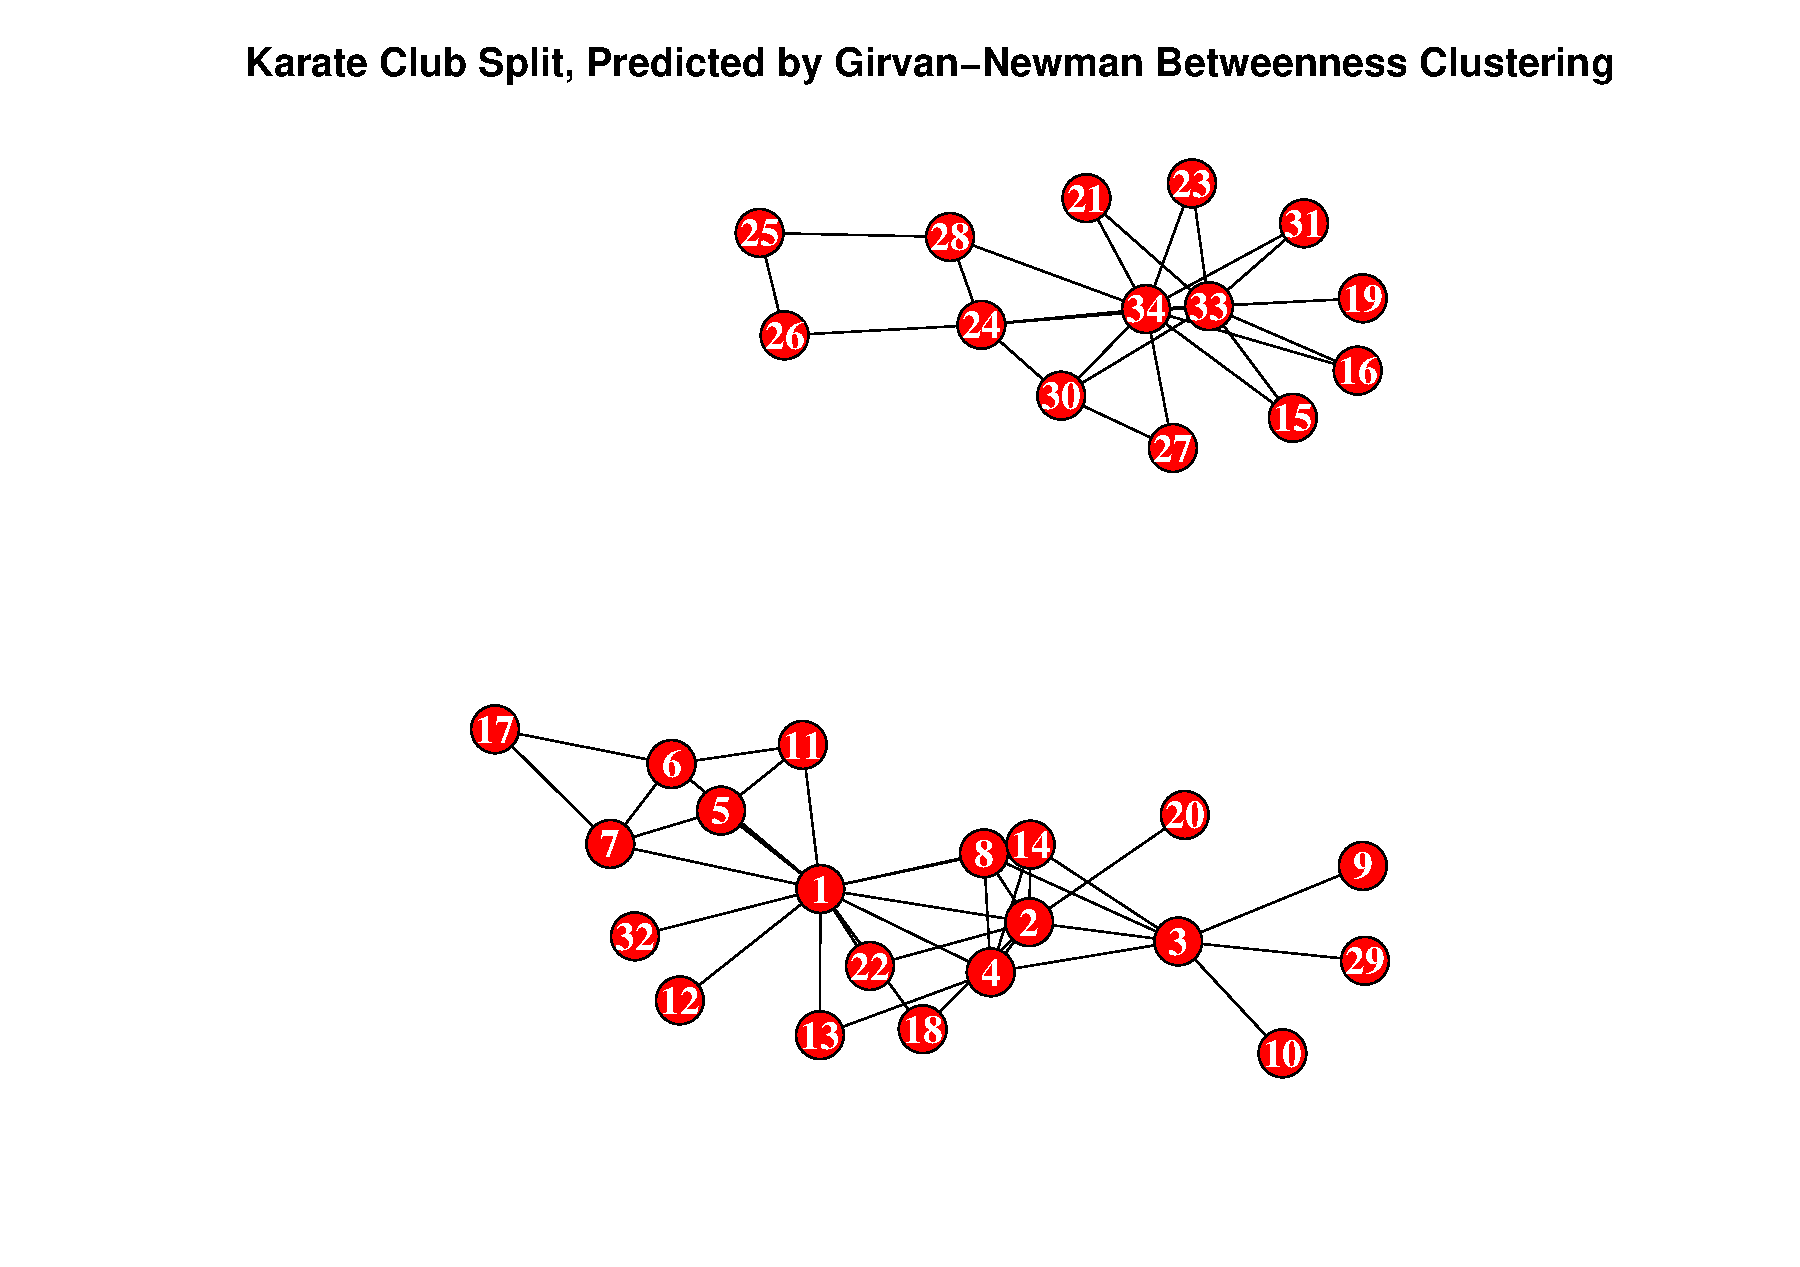
\includegraphics[scale=0.5]{club-after.pdf}
\caption{Karate Club Graph Split Predicted by Girvan \& Newman Betweenness Clustering}
\label{fig:club-after}
\end{figure}

\newpage
\lstinputlisting[language=R,frame=single,caption={R program for Girvan \& Newman Betweenness Clustering shown in Figures \ref{fig:club-before} and \ref{fig:club-after}},label=lst:q1codeR,captionpos=b,numbers=left,showspaces=false,showstringspaces=false,basicstyle=\footnotesize]{R-code/community-functions.R}

\newpage


\section*{2}

\subsection*{Question}

2.  We know the group split in two different groups.  Suppose the
disagreements in the group were more nuanced -- what would the clubs
look like if they split into groups of 3, 4, and 5?


\subsection*{Answer}

\begin{figure}[h]
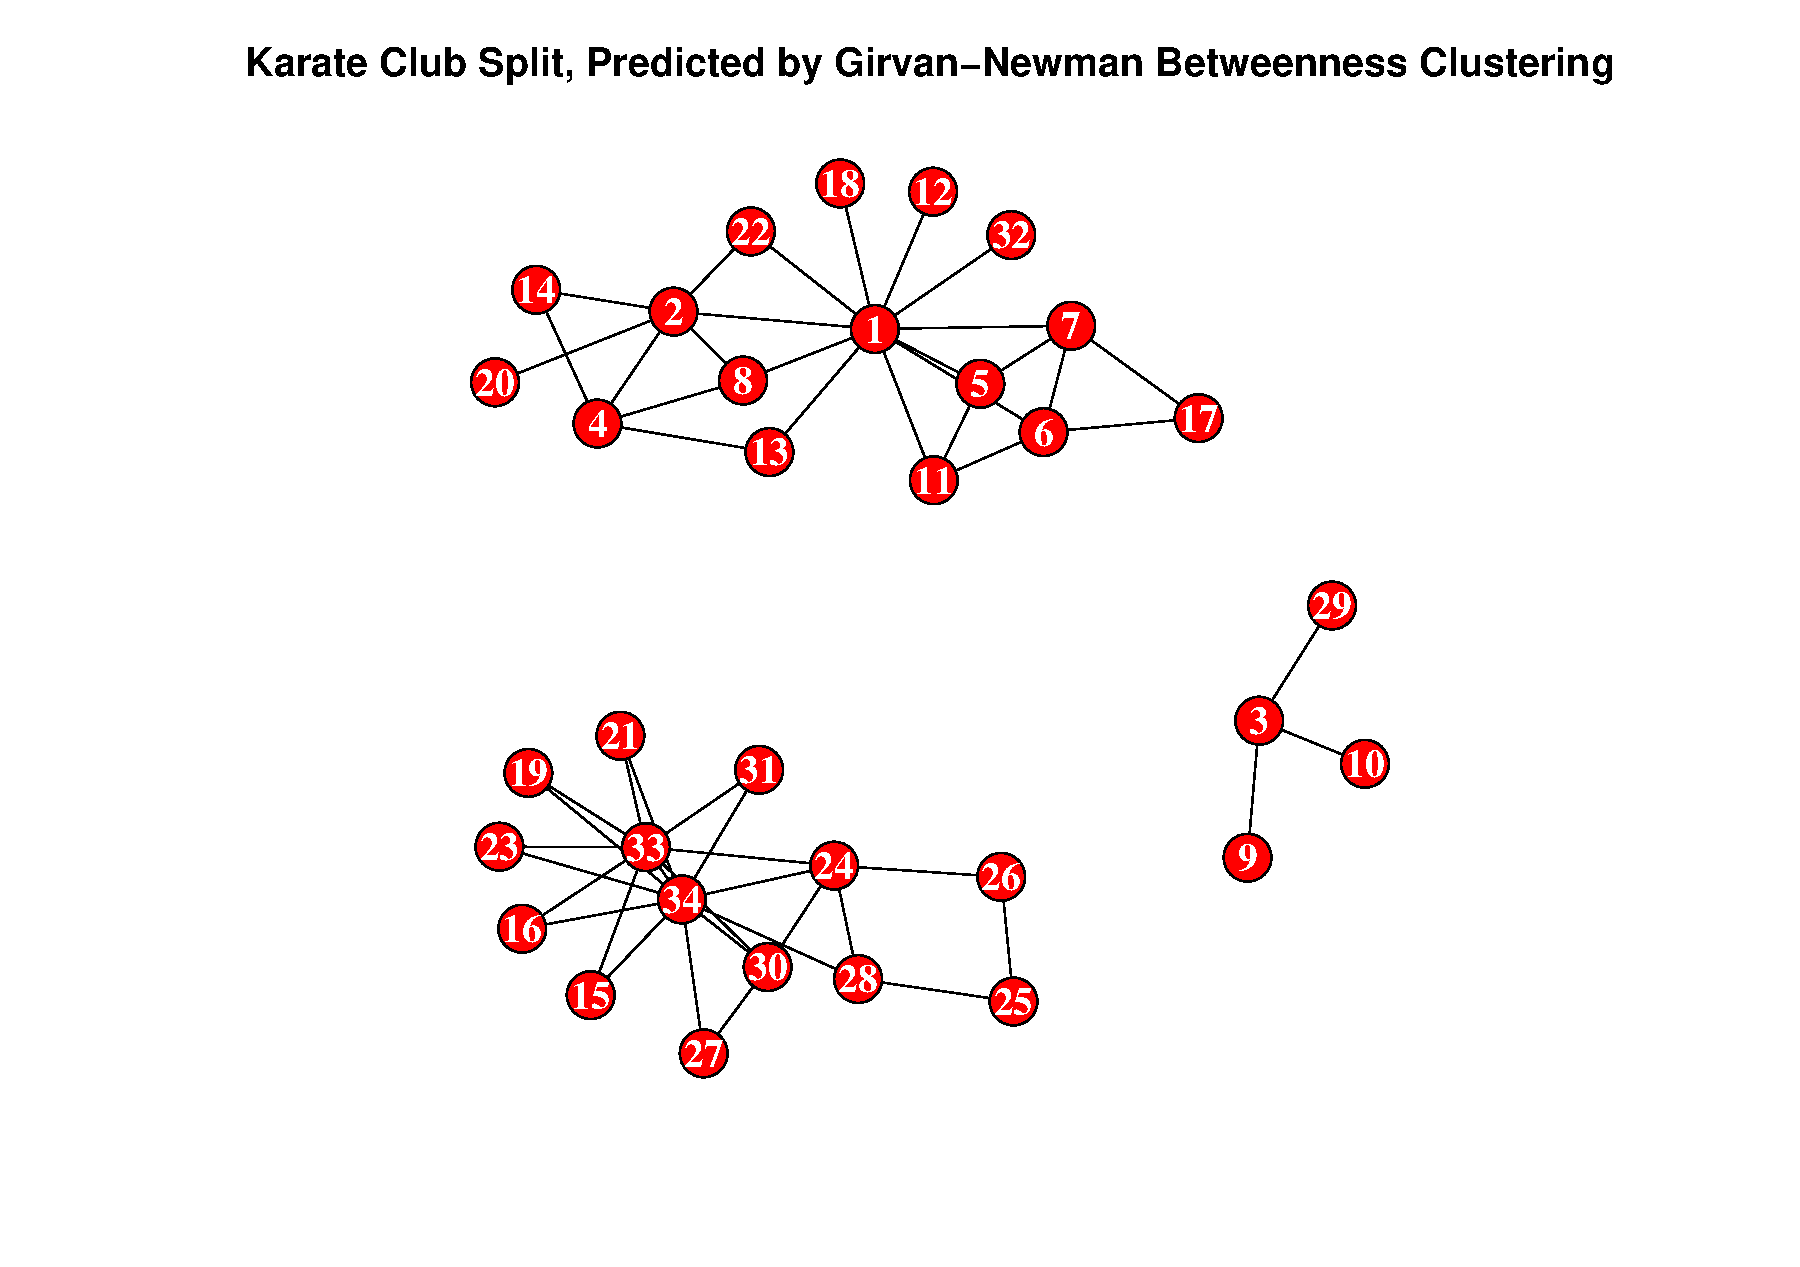
\includegraphics[scale=0.5]{group-of-3.pdf}
\caption{Karate Club Graph Split Into 3 Groups Predicted by Girvan \& Newman Betweenness Clustering}
\label{fig:club-3-split}
\end{figure}

\begin{figure}[h]
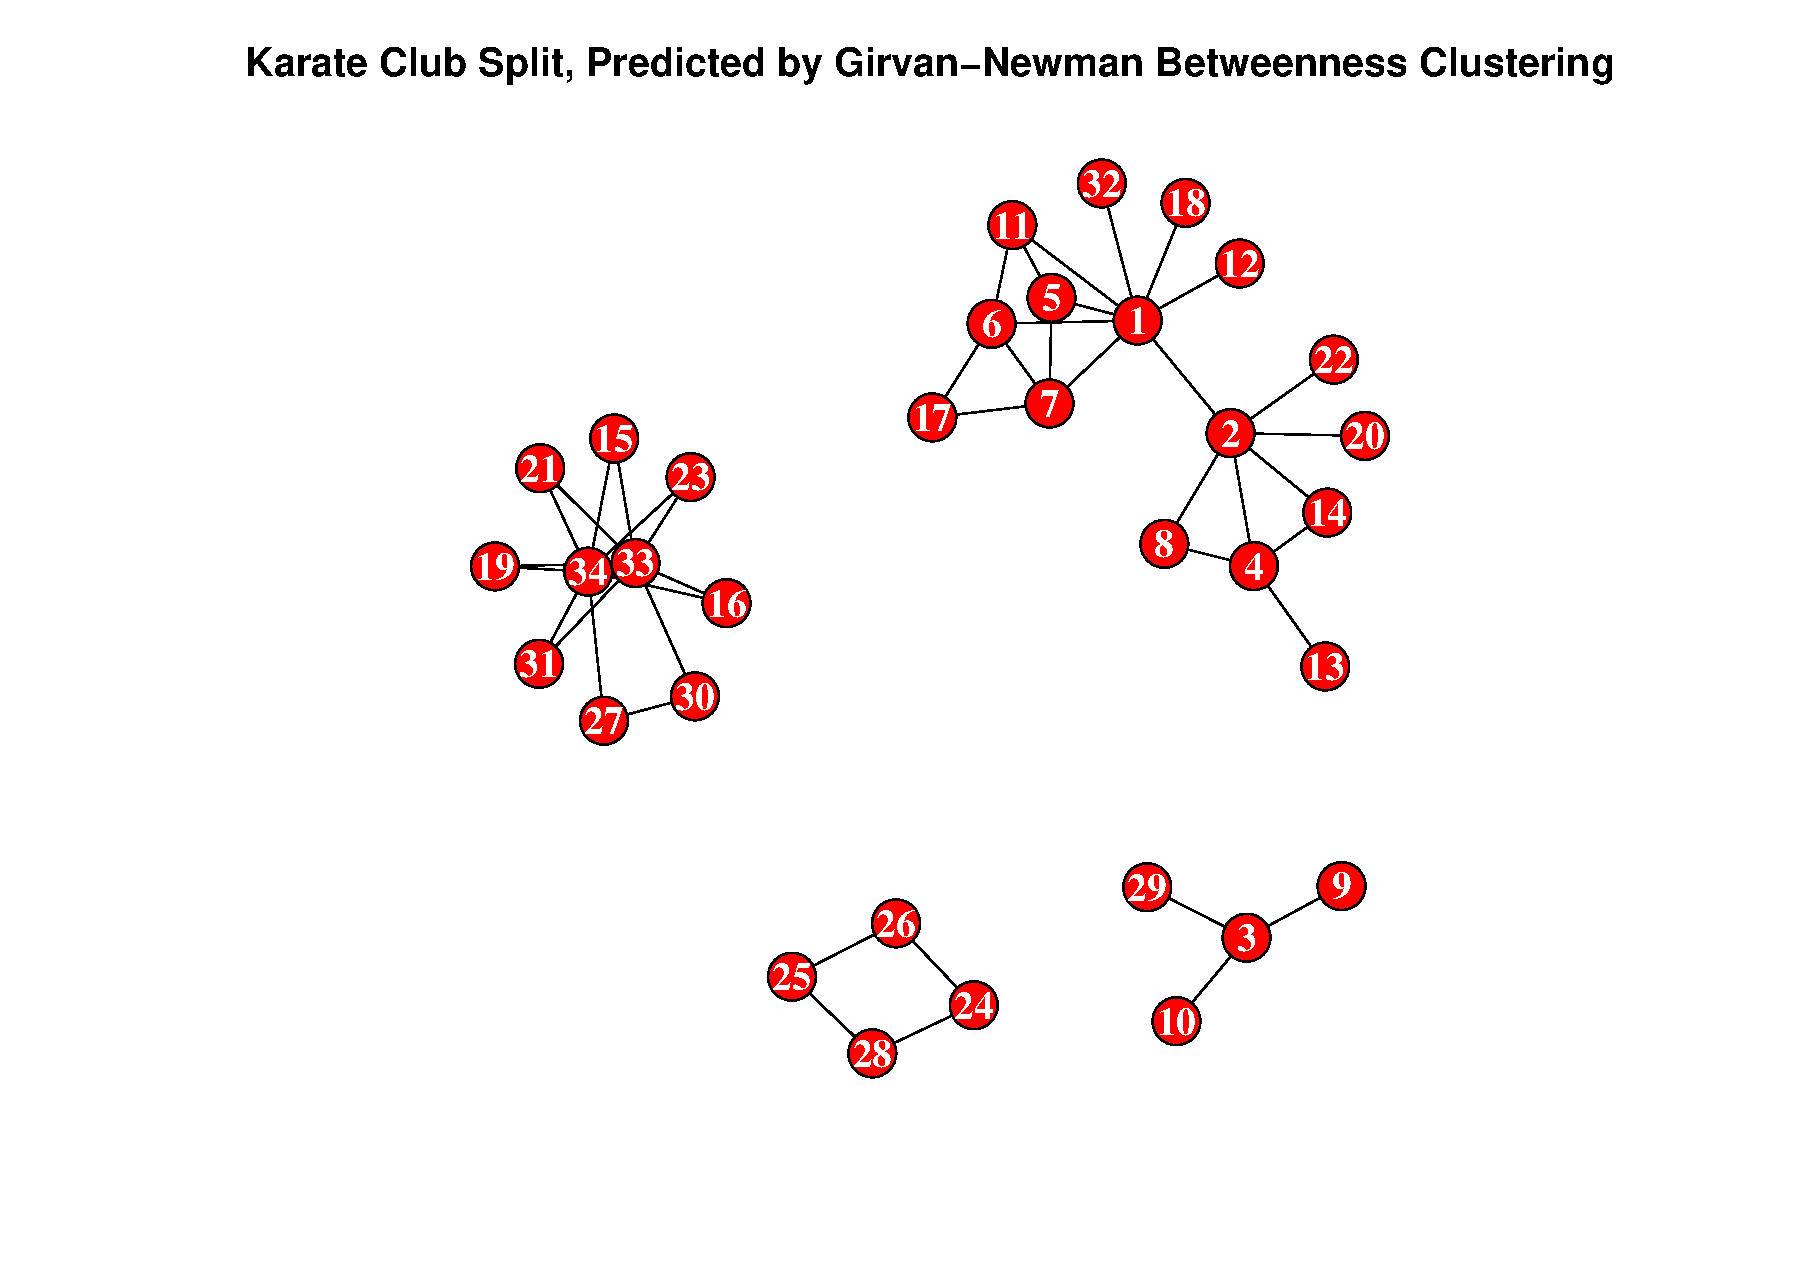
\includegraphics[scale=0.5]{group-of-4.pdf}
\caption{Karate Club Graph Split Into 4 Groups Predicted by Girvan \& Newman Betweenness Clustering}
\label{fig:club-4-split}
\end{figure}

\begin{figure}[h]
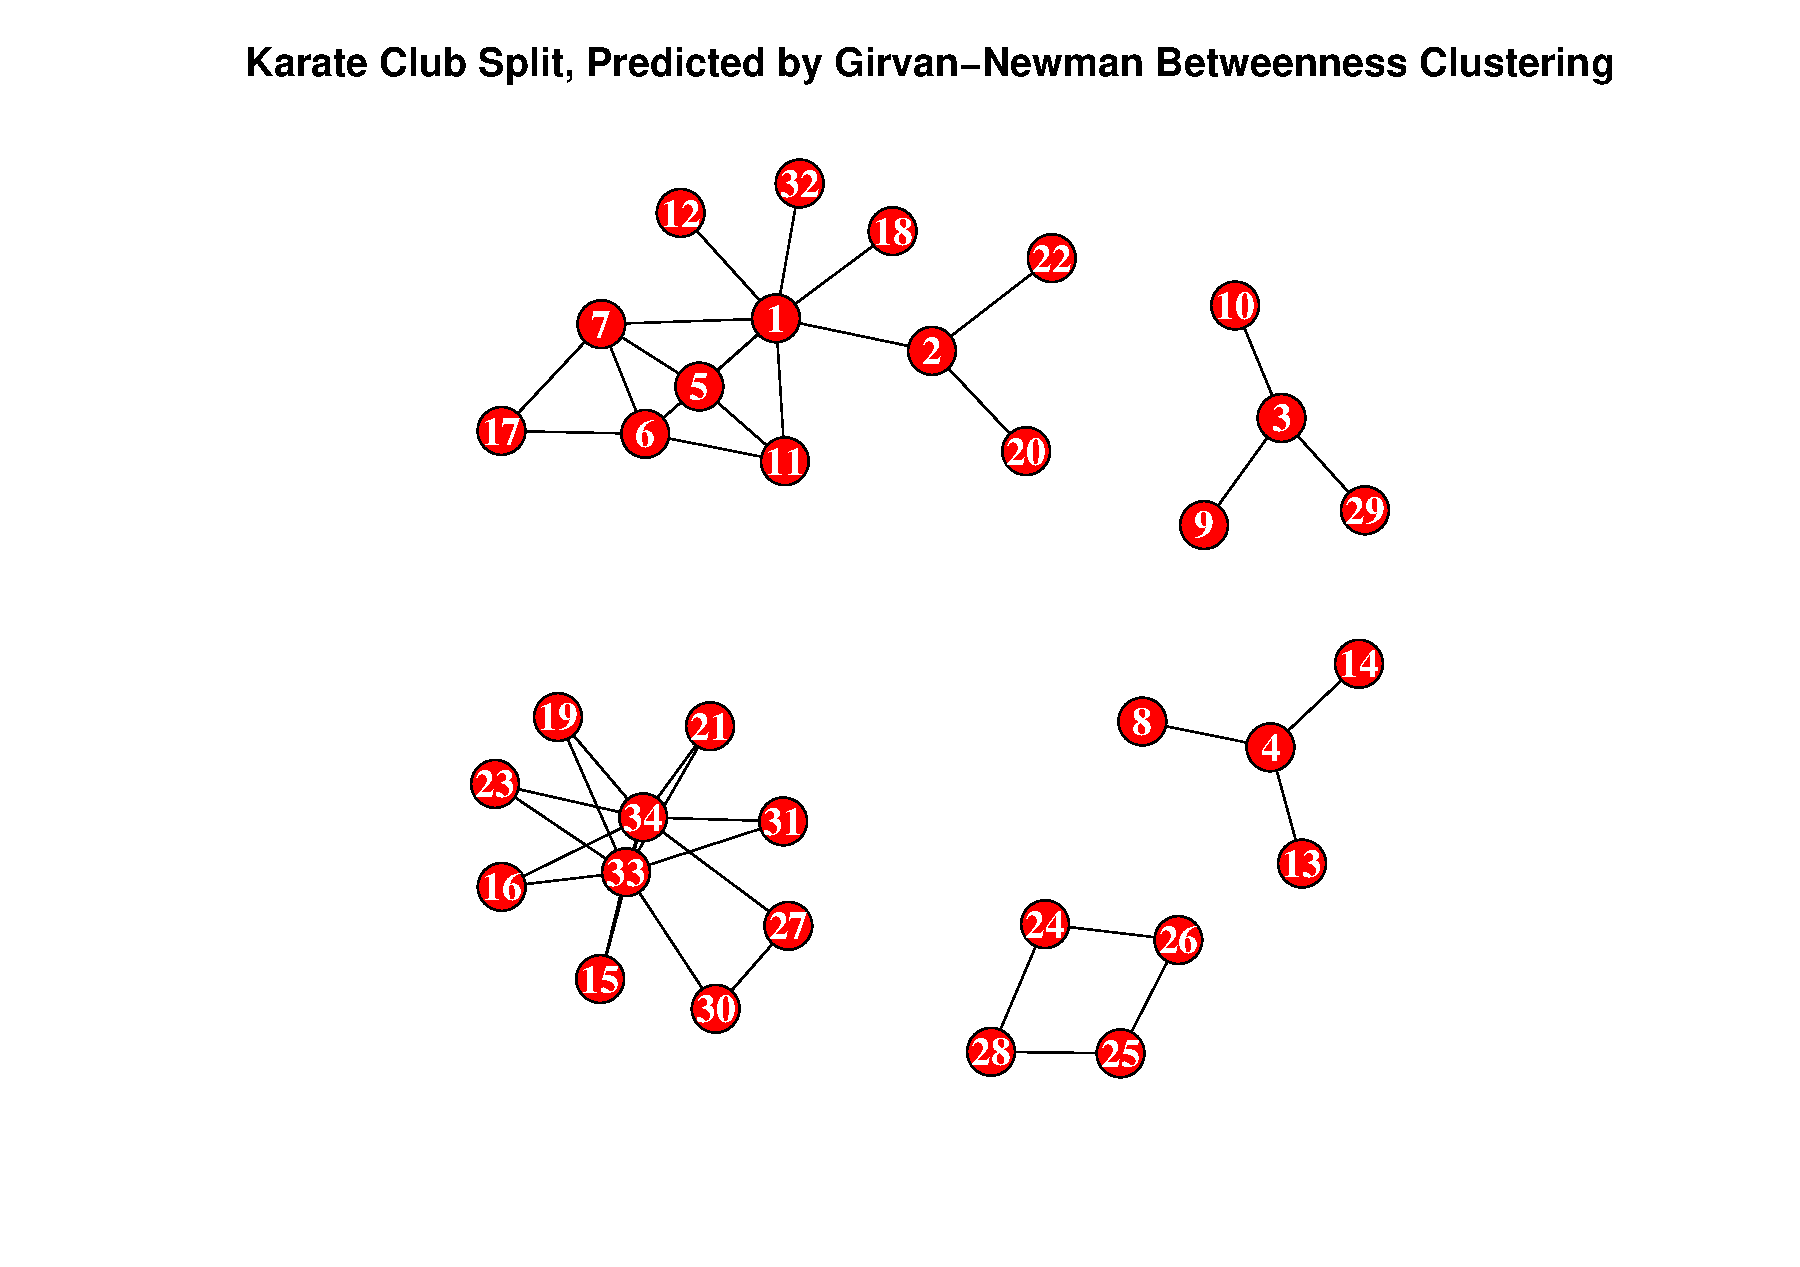
\includegraphics[scale=0.5]{group-of-5.pdf}
\caption{Karate Club Graph Split Into 5 Groups Predicted by Girvan \& Newman Betweenness Clustering}
\label{fig:club-5-split}
\end{figure}


\clearpage
\bibliographystyle{acm}
\bibliography{references}

\end{document}